% Created 2016-12-06 ter 02:35
% Intended LaTeX compiler: pdflatex
\documentclass[12pt,xcolor=dvipsnames,presentation]{beamer}
\usepackage[utf8]{inputenc}
\usepackage[T1]{fontenc}
\usepackage{graphicx}
\usepackage{grffile}
\usepackage{longtable}
\usepackage{wrapfig}
\usepackage{rotating}
\usepackage[normalem]{ulem}
\usepackage{amsmath}
\usepackage{textcomp}
\usepackage{amssymb}
\usepackage{capt-of}
\usepackage{hyperref}
\usepackage{tikz}
\usepackage{perpage}
\usetikzlibrary{arrows,shapes}
\usedescriptionitemofwidthas{bl}
\usepackage[T1]{fontenc}
\usepackage[utf8]{inputenc}
\usepackage{ifthen,graphicx,amsmath,amstext,gensymb,amssymb}
\usepackage{boxedminipage,xspace,multicol}
\usetheme{Madrid}
\usecolortheme[named=NavyBlue]{structure}
\useinnertheme{circles}
\setbeamertemplate{footline}[frame number]
\setbeamertemplate{navigation symbols}{}
\usepackage{verbments}
\usepackage{xcolor}
\usepackage{color}
\usepackage{url} \urlstyle{sf}
\usepackage[american]{babel}
\usepackage{pdfpages}
\usepackage{relsize}
\usepackage{tikzsymbols}
%\usepackage{tabularx}
%\usepackage{booktabs}
\def\smiley{\Smiley[1][green!80!white]}
\def\frowny{\Sadey[1][red!80!white]}
\def\winkey{\Winkey[1][yellow]}


% #+LATEX_HEADER: \usedescriptionitemofwidthas{bl}
% #+LATEX_HEADER: \usepackage[T1]{fontenc}
% #+LATEX_HEADER: \usepackage[utf8]{inputenc}
% #+LATEX_HEADER: \usepackage[american]{babel}
% #+LATEX_HEADER: \usepackage{ifthen,figlatex,amsmath,amstext,gensymb,amssymb}
% #+LATEX_HEADER: \usepackage{boxedminipage,xspace,multicol}
% #+LATEX_HEADER: %%%%%%%%% Begin of Beamer Layout %%%%%%%%%%%%%
% #+LATEX_HEADER: \ProcessOptionsBeamer
% #+LATEX_HEADER: \usecolortheme{whale}
% #+LATEX_HEADER: \usecolortheme[named=BrickRed]{structure}
% #+LATEX_HEADER: \useinnertheme{rounded}
% #+LATEX_HEADER: \useoutertheme{infolines}
% #+LATEX_HEADER: \setbeamertemplate{footline}[frame number]
% #+LATEX_HEADER: \setbeamertemplate{headline}[default]
% #+LATEX_HEADER: \setbeamertemplate{navigation symbols}{}
% #+LATEX_HEADER: \defbeamertemplate*{headline}{info theme}{}
% #+LATEX_HEADER: \defbeamertemplate*{footline}{info theme}{\leavevmode%
% #+LATEX_HEADER:   \hbox{%
% #+LATEX_HEADER:     \begin{beamercolorbox}[wd=.2\paperwidth,ht=2.25ex,dp=1ex,center]{author in head/foot}%
% #+LATEX_HEADER:       \usebeamerfont{author in head/foot}\insertshortauthor
% #+LATEX_HEADER:     \end{beamercolorbox}%
% #+LATEX_HEADER:   \begin{beamercolorbox}[wd=.71\paperwidth,ht=2.25ex,dp=1ex,center]{title in head/foot}%
% #+LATEX_HEADER:     \usebeamerfont{title in head/foot}\insertsectionhead
% #+LATEX_HEADER:   \end{beamercolorbox}%
% #+LATEX_HEADER:   \begin{beamercolorbox}[wd=.09\paperwidth,ht=2.25ex,dp=1ex,right]{section in head/foot}%
% #+LATEX_HEADER:     \usebeamerfont{section in head/foot}\insertframenumber{}~/~\inserttotalframenumber\hspace*{2ex} 
% #+LATEX_HEADER:   \end{beamercolorbox}
% #+LATEX_HEADER:   }\vskip0pt}
% #+LATEX_HEADER: \setbeamertemplate{footline}[info theme]
% #+LATEX_HEADER: %%%%%%%%% End of Beamer Layout %%%%%%%%%%%%%
% #+LATEX_HEADER: \usepackage{verbments}
% #+LATEX_HEADER: \usepackage{xcolor}
% #+LATEX_HEADER: \usepackage{color}
% #+LATEX_HEADER: \usepackage{url} \urlstyle{sf}


\institute[]{

\includegraphics[width=.16\textwidth]{img/gppd.png}
\hfill

\includegraphics[width=.16\textwidth]{img/inf.pdf}
\hfill

\includegraphics[width=.16\textwidth]{img/ufrgs.pdf}
\hfill

\includegraphics[width=.26\textwidth]{img/hpe.jpg}
}
\usetheme{default}
\author{Gabriel B. Moro \\ gabriel.bmoro@inf.ufrgs.br}
\date{Porto Alegre, December 2016}
\title{Retrospective: September to December}
\hypersetup{
 pdfauthor={Gabriel B. Moro \\ gabriel.bmoro@inf.ufrgs.br},
 pdftitle={Retrospective: September to December},
 pdfkeywords={},
 pdfsubject={},
 pdfcreator={Emacs 24.5.1 (Org mode 9.0)}, 
 pdflang={English}}
\begin{document}

\maketitle

\let\alert=\structure % to make sure the org * * works
\def\n{\\\hline}             
\def\eg{e.g.,\xspace}
\def\Eg{E.g.,\xspace}
\def\ie{i.e.,\xspace}
\let\alert=\structure
\let\epsilon=\varepsilon
%\let\leq=\leqslant
%\let\geq=\geqslant
\def\R{\ensuremath{\mathbb{R}}\xspace}
\def\F{\ensuremath{\mathcal{F}}\xspace}
\def\N{\ensuremath{\mathcal{N}}\xspace}
\def\P{\ensuremath{\operatorname{P}}\xspace}
\def\E{\ensuremath{\operatorname{E}}\xspace}
\def\Var{\ensuremath{\operatorname{Var}}\xspace}
\def\rv#1{\ensuremath{\textcolor{blue}{#1}}\xspace} % DarkBlue

\def\RR{\ensuremath{R^2}\xspace}


\makeatletter
\gdef\fsvtpage{\ps@navigation\refstepcounter{framenumber}}%
\makeatother
\setbeamercolor{background canvas}{bg=}

\definecolor{keywords}{RGB}{255,0,90}
\definecolor{comments}{RGB}{60,179,113}
\definecolor{fore}{RGB}{249,242,215}
\definecolor{back}{RGB}{51,51,51}
\newcommand{\accolade}[1]{$\left\{\begin{array}{c}\vspace{#1}\end{array}\right.$}
%\lstset{
%  basicstyle=\color{fore},
%  keywordstyle=\color{keywords},
%  commentstyle=\color{comments},
%  backgroundcolor=\color{back}
%}

\newcommand{\restorefootline}{\setbeamertemplate{navigation symbols}{}}
\newcommand{\setfootline}[1]{\setbeamertemplate{navigation symbols}{\textcolor{black}{\textbf{#1}}}}
\newcommand{\includeslides}[3]{%
  \setfootline{#1}%
  \includepdf[pages={#2},pagecommand={\fsvtpage},turn=false,noautoscale=false,column=false,columnstrict=false,openright=false]{pdf_sources/#3}%
%  \includepdf[pages={#2},pagecommand={\fsvtpage},scale=.8,offset=20
%  -23,turn=false,noautoscale=false,column=false,columnstrict=false,openright=false]{pdf_sources/#3}%
  \restorefootline%
}
\end

\def\recurrenttoc{%
\makeatletter
\AtBeginSection[]
{
  \frame<handout:0>
  {
    \frametitle{Outline}
    \tableofcontents[current,currentsubsection]
  }
}
\makeatother
}

\newcommand{\bottomcite}[1]{\fbox{\vbox{\footnotesize #1}}}

\newcommand{\prettysmall}[1]{\fontsize{#1}{#1}\selectfont}

\tikzstyle{format} = [draw, thin, fill=blue!20]
\tikzstyle{medium} = [ellipse, draw, thin, fill=green!20, minimum height=2.5em]


\section{Methodology}
\label{sec:orgc6d22b7}
\subsection{}
\label{sec:orgc6e988b}
\begin{frame}[label={sec:orgc179854}]{Methodology}
\begin{tikzpicture}

\node at (0,17) [draw,rectangle,rectangle left angle=70,rectangle right angle=-70,minimum height=1cm, fill=orange!20] (App) {App};
\node at (2.4,18) [draw,rectangle split, rectangle split horizontal,rectangle split parts=3,minimum height=1cm,fill=gray!10] (Lik) {\nodepart{two}\shortstack{Likwid\\}};
\node at (2.4,16) [draw,rectangle split, rectangle split horizontal,rectangle split parts=3,minimum height=1cm,fill=gray!10] (Sc) {\nodepart{two}\shortstack{Score-p\\}};
\node at (5.4,18) [draw,trapezium,trapezium left angle=70,trapezium right angle=-70,minimum height=1cm] (T1) {Trace};
\node at (5.4,16) [draw,trapezium,trapezium left angle=70,trapezium right angle=-70,minimum height=1cm] (T2) {Trace};
\node at (9.4,17) [draw,rectangle,rectangle left angle=70,rectangle right angle=-70,minimum height=1cm,rounded corners,fill=green!20] (Det){\shortstack{Detect Memory-Bound\\ Regions}};

\draw[->] (App.east) + (-1,1.1) coordinate (a1) ++ (0.02,0.12) -- (Lik.west |- a1);
\draw[->] (App.east) + (-1,-0.9) coordinate (a1) ++ (0.02,0.12) -- (Sc.west |- a1);
\draw[->] (Lik.west) + (2.35,0.02) coordinate (a1) -- (T1.west |- a1);
\draw[->] (Sc.west) + (2.52,0.02) coordinate (a1) -- (T2.west |- a1);
\draw[->] (T1.east) + (-1,-0.3) coordinate (a1) ++ (0.02,0.12) -- (Det.west |- a1);
\draw[->] (T2.east) + (-1,0.4) coordinate (a1) ++ (0.02,0.12) -- (Det.west |- a1);


\end{tikzpicture}
\end{frame}

\begin{frame}[fragile,label={sec:org3d3b3e2}]{Use of the Likwid}
 \begin{columns}\begin{column}{.45\linewidth}
\begin{figure}[!htb]
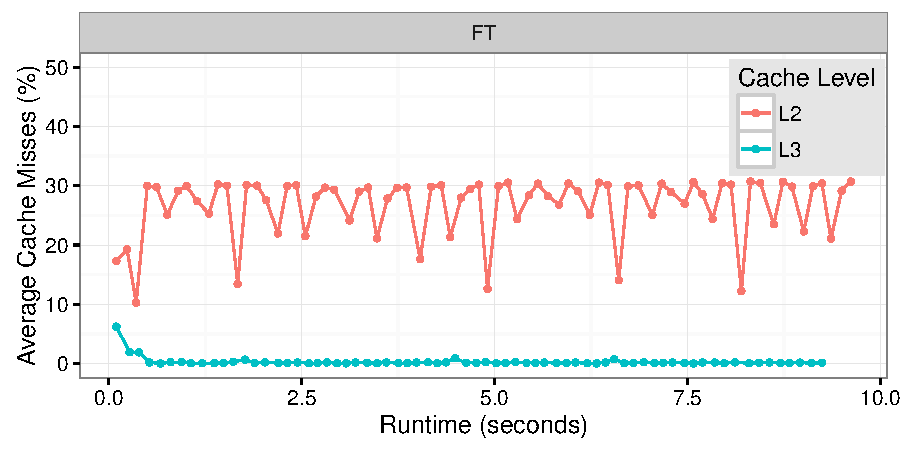
\includegraphics[width=\linewidth]{../../producao/2016_wsppd/img/ft_L2_L3_100ms.pdf}
\caption{Sampling interval - 100 milliseconds$^{[1]}$.}
\label{figFT}
\end{figure}

\end{column}
\begin{column}{.35\linewidth}
{\small
\texttt{Beagle1:}
\begin{itemize}
\item 2 x Intel (R) Xeon (R) E5-2650 CPU 2.00 GHz
\begin{itemize}
\item 8 physical cores
\item Hyper-Threading tecnology
\end{itemize}
\end{itemize}
}
\end{column}
\end{columns}

\vspace{2cm}
\hline
\vspace{0.2cm}
\tiny \(^{[1]}\) \alert{Moro, Gabriel and Schnorr, Lucas}. \emph{Measuring Hardware Counters for
HPC Application Phase Detection}. XIV Workshop de Processamento
Paralelo e Distribuído. Porto Alegre, 2016.
\end{frame}

\begin{frame}[fragile,label={sec:orgd1f265d}]{Use of the Likwid}
 \begin{columns}\begin{column}{.45\linewidth}
\begin{figure}[!htb]
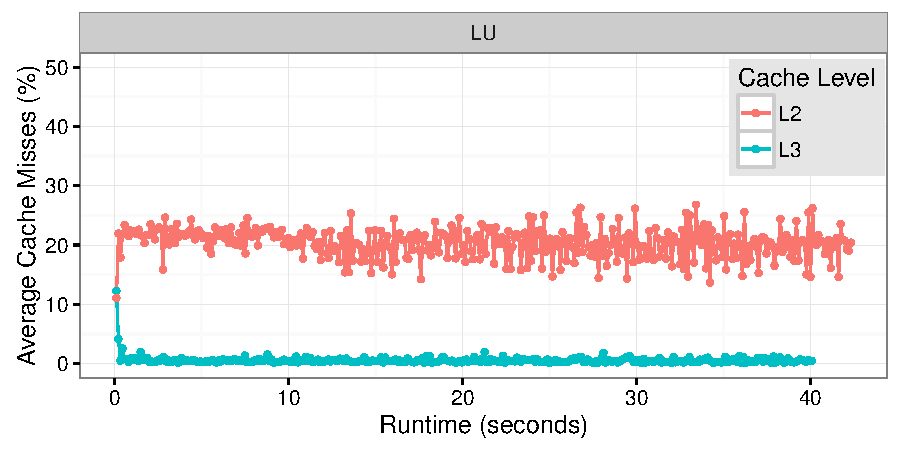
\includegraphics[width=\linewidth]{../../producao/2016_wsppd/img/lu_L2_L3_100ms.pdf}
\caption{Sampling interval - 100 milliseconds$^{[1]}$.}
\label{figFT}
\end{figure}

\end{column}
\begin{column}{.35\linewidth}
{\small
\texttt{Beagle1:}
\begin{itemize}
\item 2 x Intel (R) Xeon (R) E5-2650 CPU 2.00 GHz
\begin{itemize}
\item 8 physical cores
\item Hyper-Threading tecnology
\end{itemize}
\end{itemize}
}
\end{column}
\end{columns}

\vspace{2cm}
\hline
\vspace{0.2cm}
\tiny \(^{[1]}\) \alert{Moro, Gabriel and Schnorr, Lucas}. \emph{Measuring Hardware Counters for
HPC Application Phase Detection}. XIV Workshop de Processamento
Paralelo e Distribuído. Porto Alegre, 2016.
\end{frame}
\end{document}